\documentclass[11pt,
  english,
  a4paper,
]{article}
\usepackage{sa4ss}
\usepackage{amsmath,amssymb,array}
\usepackage{booktabs}

% From tagged-template.latex
\usepackage{lmodern}
\usepackage{ifxetex,ifluatex}
\ifnum 0\ifxetex 1\fi\ifluatex 1\fi=0 % if pdftex
  \usepackage[T1]{fontenc}
  \usepackage[utf8]{inputenc}
  \usepackage{textcomp} % provide euro and other symbols
\else % if luatex or xetex
  \usepackage{unicode-math}
  \defaultfontfeatures{Scale=MatchLowercase}
  \defaultfontfeatures[\rmfamily]{Ligatures=TeX,Scale=1}
\fi

% Use upquote if available, for straight quotes in verbatim environments
\IfFileExists{upquote.sty}{\usepackage{upquote}}{}
\IfFileExists{microtype.sty}{% use microtype if available
  \usepackage[]{microtype}
  \UseMicrotypeSet[protrusion]{basicmath} % disable protrusion for tt fonts
}{}
\makeatletter
\@ifundefined{KOMAClassName}{% if non-KOMA class
  \IfFileExists{parskip.sty}{%
    \usepackage{parskip}
  }{% else
    \setlength{\parindent}{0pt}
    \setlength{\parskip}{6pt plus 2pt minus 1pt}}
}{% if KOMA class
  \KOMAoptions{parskip=half}}
\makeatother
\usepackage{xcolor}
\IfFileExists{xurl.sty}{\usepackage{xurl}}{} % add URL line breaks if available
\hypersetup{
  pdftitle={Status of Quillback Rockfish (Sebastes maliger) along the Oregon US West coast in 2021},
  pdflang={en},
  hidelinks,
  pdfcreator={LaTeX via pandoc}}
\urlstyle{same} % disable monospaced font for URLs
\usepackage{longtable}
% Correct order of tables after \paragraph or \subparagraph
\usepackage{etoolbox}
\makeatletter
\patchcmd\longtable{\par}{\if@noskipsec\mbox{}\fi\par}{}{}
\makeatother
% Allow footnotes in longtable head/foot
\IfFileExists{footnotehyper.sty}{\usepackage{footnotehyper}}{\usepackage{footnote}}
\makesavenoteenv{longtable}
\usepackage{graphicx}
\makeatletter
\def\maxwidth{\ifdim\Gin@nat@width>\linewidth\linewidth\else\Gin@nat@width\fi}
\def\maxheight{\ifdim\Gin@nat@height>\textheight\textheight\else\Gin@nat@height\fi}
\makeatother
% Scale images if necessary, so that they will not overflow the page
% margins by default, and it is still possible to overwrite the defaults
% using explicit options in \includegraphics[width, height, ...]{}
\setkeys{Gin}{width=\maxwidth,height=\maxheight,keepaspectratio}
% Set default figure placement to htbp
\makeatletter
\def\fps@figure{htbp}
\makeatother
\setlength{\emergencystretch}{3em} % prevent overfull lines
\providecommand{\tightlist}{%
  \setlength{\itemsep}{0pt}\setlength{\parskip}{0pt}}
\setcounter{secnumdepth}{5}
\ifxetex
  % Load polyglossia as late as possible: uses bidi with RTL langages (e.g. Hebrew, Arabic)
  \usepackage{polyglossia}
  \setmainlanguage[]{english}
\else
  \usepackage[shorthands=off,main=english]{babel}
\fi

\providecommand{\tightlist}{%
  \setlength{\itemsep}{0pt}\setlength{\parskip}{0pt}}


\date{}
\newcommand{\trTitle}{Status of Quillback Rockfish (\emph{Sebastes maliger}) along the Oregon US West coast in 2021}
\newcommand{\trYear}{2021}
\newcommand{\trMonth}{February}
\newcommand{\trAuthsLong}{true}
\newcommand{\trAuthsBack}{Langseth, B.J., C.R. Wetzel, J.M. Cope, A.D. Whitman}
\newcommand{\trCitation}{
\begin{hangparas}{1em}{1}
\trAuthsBack{}. \trYear{}. \trTitle{}. Pacific Fisheries Management Council, Portland, Oregon. \pageref{LastPage}{}\,p.
\end{hangparas}}

\AtBeginDocument{\tagstructbegin{tag=Document}}
\AtEndDocument{\tagstructend}
\pretocmd{\maketitle}{\tagstructbegin{tag=H1}\tagmcbegin{tag=H1}}{}{}
\apptocmd{\maketitle}{\tagmcend\tagstructend}{}{}

\begin{document}

%%%%% Frontmatter %%%%%

% Footnote symbols in front matter
\renewcommand*{\thefootnote}{\fnsymbol{footnote}}

\small
\thispagestyle{empty}
\pagenumbering{roman}
\noindent
\begin{center}
\title{Status of Quillback Rockfish (\emph{Sebastes maliger}) along the Oregon US West coast in 2021}
% \textnormal{\MakeTextUppercase{\trTitle{}}}
\vspace{1.5cm}
{\Large\textbf\newline{Status of Quillback Rockfish (\emph{Sebastes maliger}) along the Oregon US West coast in 2021}}
\vfill
by\\
Brian J. Langseth\textsuperscript{1}\\
Chantel R. Wetzel\textsuperscript{1}\\
Jason M. Cope\textsuperscript{1}\\
Alison D. Whitman\textsuperscript{2}\vfill
\textsuperscript{1}Northwest Fisheries Science Center, U.S. Department of Commerce, National Oceanic and Atmospheric Administration, National Marine Fisheries Service, 2725 Montlake Boulevard East, Seattle, Washington 98112\\
\textsuperscript{2}Oregon Department of Fish and Wildlife, 2040 Southeast Marine Science Drive, Newport, Oregon 97365\vfill
\trMonth{} \trYear{}
\end{center}
\clearpage

% Fourth page: Colophon
\thispagestyle{empty}
\vspace*{\fill}
\begin{center}
\copyright{} Pacific Fisheries Management Council, \trYear{}\\
\end{center}
\par
\bigskip
\noindent
Correct citation for this publication:
\bigskip
\par
\trCitation{}
\clearpage

% Add TOC to pdf bookmarks (clickable pdf)
\pdfbookmark[1]{\contentsname}{toc}

% Table of contents page, lists of figures and tables
\tableofcontents\clearpage
\listoffigures \listoftables \clearpage
\label{TRlastRoman}
\clearpage

% Table of contents
\newpage
\thispagestyle{empty} % to remove page number

% Settings for the main document
\pagenumbering{arabic}  % Regular page numbers
\pagestyle{plain}  % No page number on first page of main document, use 'empty'
\renewcommand*{\thefootnote}{\arabic{footnote}}  % Back to numeric footnotes
\setcounter{footnote}{0}  % And start at 1
\renewcommand{\headrulewidth}{0.5pt}
\renewcommand{\footrulewidth}{0.5pt}
%\pagestyle{fancy}\fancyhead[c]{Draft: Do not cite or circulate}

\newcommand{\lt}{\ensuremath <}
\newcommand{\gt}{\ensuremath >}

%Define cslreferences environment, required by pandoc 2.8
%https://github.com/rstudio/rmarkdown/issues/1649

\pagebreak
\setlength{\parskip}{5mm plus1mm minus1mm}
\pagenumbering{arabic}
\setcounter{page}{1}
\renewcommand{\thefigure}{\arabic{figure}}
\renewcommand{\thetable}{\arabic{table}}
\setcounter{table}{0}
\setcounter{figure}{0}

\tagstructbegin{tag=H1}\tagmcbegin{tag=H1}

\hypertarget{introduction}{%
\section{Introduction}\label{introduction}}

\leavevmode\tagmcend\tagstructend

\tagstructbegin{tag=H2}\tagmcbegin{tag=H2}

\hypertarget{basic-information}{%
\subsection{Basic Information}\label{basic-information}}

\leavevmode\tagmcend\tagstructend

\tagstructbegin{tag=P}\tagmcbegin{tag=P}

This assessment reports the status of quillback rockfish (\emph{Sebastes maliger}) off the U.S. West Coast using data through 2020. Quillback rockfish is a medium- to large-sized nearshore rockfish found from California to the Gulf of Alaska {\tagstructbegin{tag=Reference}\tagmcbegin{tag=Reference}({\textbf{???}})\leavevmode\tagmcend\tagstructend}. Off the U.S. West Coast quillback rockfish are primarily located north of central California, with rare observations south of Point Conception.

\leavevmode\tagmcend\tagstructend\par

\tagstructbegin{tag=P}\tagmcbegin{tag=P}

The stock off the Oregon coast was assessed as a separate stock from other populations off the U.S. West Coast based on the fairly sedentary nature of quillback rockfish which likely limits flow of fish between California and Washington {\tagstructbegin{tag=Reference}\tagmcbegin{tag=Reference}({\textbf{???}}; {\textbf{???}})\leavevmode\tagmcend\tagstructend}. The substrate of the southern Washington coast is typically sandy bottom, which creates a natural separation between the Oregon and Washington populations. Additionally, the exploitation history and magnitude of removals off the Oregon coast differ from those in Washington and California.

\leavevmode\tagmcend\tagstructend\par

\tagstructbegin{tag=H2}\tagmcbegin{tag=H2}

\hypertarget{life-history}{%
\subsection{Life History}\label{life-history}}

\leavevmode\tagmcend\tagstructend

\tagstructbegin{tag=P}\tagmcbegin{tag=P}

Quillback rockfish are found in waters less than 274 meters in depth in nearshore kelp forests and rocky habitat {\tagstructbegin{tag=Reference}\tagmcbegin{tag=Reference}({\textbf{???}})\leavevmode\tagmcend\tagstructend}. The diets of quillback rockfish consist primarily of crustaceans, mollusks, and fish {\tagstructbegin{tag=Reference}\tagmcbegin{tag=Reference}({\textbf{???}}; {\textbf{???}})\leavevmode\tagmcend\tagstructend}. The body coloring or quillback rockfish varies across the coast with northern fish often exhibiting dark brown to olive with southern fish exhibiting yellow to olive-pink variations in color {\tagstructbegin{tag=Reference}\tagmcbegin{tag=Reference}({\textbf{???}})\leavevmode\tagmcend\tagstructend} which initially led to them being designated as two separate species (\emph{S. caurinus} and \emph{S. vexillaris}).

\leavevmode\tagmcend\tagstructend\par

\tagstructbegin{tag=P}\tagmcbegin{tag=P}

Limited studies have been performed looking for genetic variation in quillback rockfish across the U.S. West Coast. Genetic work has revealed significant differences between Puget Sound and coastal stocks of quillback rockfish {\tagstructbegin{tag=Reference}\tagmcbegin{tag=Reference}({\textbf{???}}; {\textbf{???}})\leavevmode\tagmcend\tagstructend}, however {\tagstructbegin{tag=Reference}\tagmcbegin{tag=Reference}({\textbf{???}})\leavevmode\tagmcend\tagstructend} did not find significant differentiation in populations of quillback rockfish between Washington and Alaska when Puget Sound samples were excluded. Significant population sub-division along the U.S. West Coast has been detected for the similar, and more well-studied copper rockfish (\emph{Sebastes caurinus}), indicating limited oceanographic exchange among geographically proximate locations {\tagstructbegin{tag=Reference}\tagmcbegin{tag=Reference}({\textbf{???}}; {\textbf{???}}; {\textbf{???}})\leavevmode\tagmcend\tagstructend}. High site-fidelity {\tagstructbegin{tag=Reference}\tagmcbegin{tag=Reference}({\textbf{???}})\leavevmode\tagmcend\tagstructend} and relatively small home ranges {\tagstructbegin{tag=Reference}\tagmcbegin{tag=Reference}({\textbf{???}})\leavevmode\tagmcend\tagstructend} for quillback rockfish would suggest similar patterns of isolation-by-distance as found for other rockfish.

\leavevmode\tagmcend\tagstructend\par

\tagstructbegin{tag=P}\tagmcbegin{tag=P}

Quillback rockfish are a long-lived rockfish and estimated to live at least 90 years {\tagstructbegin{tag=Reference}\tagmcbegin{tag=Reference}(Love 1996)\leavevmode\tagmcend\tagstructend}, with estimates from Canadian waters as high as 95 years {\tagstructbegin{tag=Reference}\tagmcbegin{tag=Reference}({\textbf{???}})\leavevmode\tagmcend\tagstructend}. Quillback rockfish was determined to have a vulnerability (V = 2.22) of major concern in a productivity susceptibility analysis {\tagstructbegin{tag=Reference}\tagmcbegin{tag=Reference}({\textbf{???}})\leavevmode\tagmcend\tagstructend}.

\leavevmode\tagmcend\tagstructend\par

\tagstructbegin{tag=H2}\tagmcbegin{tag=H2}

\hypertarget{ecosystem-considerations}{%
\subsection{Ecosystem Considerations}\label{ecosystem-considerations}}

\leavevmode\tagmcend\tagstructend

\tagstructbegin{tag=P}\tagmcbegin{tag=P}

Replace text.

\leavevmode\tagmcend\tagstructend\par

\tagstructbegin{tag=H2}\tagmcbegin{tag=H2}

\hypertarget{historical-and-current-fishery-information}{%
\subsection{Historical and Current Fishery Information}\label{historical-and-current-fishery-information}}

\leavevmode\tagmcend\tagstructend

\tagstructbegin{tag=P}\tagmcbegin{tag=P}

Off the coast of Oregon quillback rockfish is primarily caught in both the commercial and recreational fisheries. The landings from the commercial fishery extend back to 1892 and other than an increase in the late 1930s through the 1940s, were minimal until the late-1960s. Currently, quillback rockfish is landed as part of both the live and dead commercial fishery off the coast of Oregon. Landings from the recreational fishery off the coast of Oregon begun in 1979 and removals from the recreational fleet have increased across time and now represent the majority of landings for quillback rockfish off the coast of Oregon. Recreational landings were large in the year that data were first available, and were expected to be minmal prior to the 1970s. Consequently a linear ramp in recreational landings was applied from 1970 to 1979.

\leavevmode\tagmcend\tagstructend\par

\tagstructbegin{tag=H2}\tagmcbegin{tag=H2}

\hypertarget{summary-of-management-history-and-performance}{%
\subsection{Summary of Management History and Performance}\label{summary-of-management-history-and-performance}}

\leavevmode\tagmcend\tagstructend

\tagstructbegin{tag=P}\tagmcbegin{tag=P}

Quillback rockfish is managed by the Pacific Fishery Management Council (PFMC) as a part of the Minor Nearshore Rockfish North and Minor Nearshore Rockfish South complexes. The North and South complexes are split at N. 40{\tagstructbegin{tag=Formula}\tagmcbegin{tag=Formula}\(^\circ\)\leavevmode\tagmcend\tagstructend} 10' Lat. N. off the U.S. West Coast. Each complex is managed based on a complex-level overfishing limit (OFL) and annual catch limit (ACL). The OFL and ACL values for the complexes are determined by summing the species specific OFLs and ACLs managed within each complex. Removals for species within each Nearshore complex are managed and tracked against the complex total OFL and ACL, rather than on a species by species basis.

\leavevmode\tagmcend\tagstructend\par

\tagstructbegin{tag=P}\tagmcbegin{tag=P}

Quillback rockfish was most recently assessed in 2010 using Depletion-Based Stock Reduction Analysis (DB-SRA) to provide estimates of coastwide OFLs ({\tagstructbegin{tag=Reference}\tagmcbegin{tag=Reference}({\textbf{???}})\leavevmode\tagmcend\tagstructend}). The coastwide OFL was then apportioned to each management area based on the proportion of historical catches North and South of 40{\tagstructbegin{tag=Formula}\tagmcbegin{tag=Formula}\(^\circ\)\leavevmode\tagmcend\tagstructend} 10' Lat. N. Assuming that current depletion was at the management target on average (e.g.~40\%), the 2010 assessment found that quillback rockfish had a 52\% chance of experiencing overfishing, in that recent coastwide catch of `r spp' slightly exceeded the median coastwide OFL estimate.

\leavevmode\tagmcend\tagstructend\par

\tagstructbegin{tag=P}\tagmcbegin{tag=P}

The current OFL and ACLs for quillback rockfish North of 40{\tagstructbegin{tag=Formula}\tagmcbegin{tag=Formula}\(^\circ\)\leavevmode\tagmcend\tagstructend} 10' Lat. N., the state/specific ACL allocation (58.4\% for Oregon; Groundfish Management Team, pers. comm.), and the total removals are shown in Table \ref{tab:ofl}.

\leavevmode\tagmcend\tagstructend\par

\tagstructbegin{tag=H2}\tagmcbegin{tag=H2}

\hypertarget{foreign-fisheries}{%
\subsection{Foreign Fisheries}\label{foreign-fisheries}}

\leavevmode\tagmcend\tagstructend

\tagstructbegin{tag=P}\tagmcbegin{tag=P}

Replace text.

\leavevmode\tagmcend\tagstructend\par

\tagstructbegin{tag=H1}\tagmcbegin{tag=H1}

\hypertarget{data}{%
\section{Data}\label{data}}

\leavevmode\tagmcend\tagstructend

\tagstructbegin{tag=P}\tagmcbegin{tag=P}

A description of each data source is provided below (Figure \ref{fig:data-plot}).

\leavevmode\tagmcend\tagstructend\par

\tagstructbegin{tag=H2}\tagmcbegin{tag=H2}

\hypertarget{fishery-dependent-data}{%
\subsection{Fishery-Dependent Data}\label{fishery-dependent-data}}

\leavevmode\tagmcend\tagstructend

\tagstructbegin{tag=H3}\tagmcbegin{tag=H3}

\hypertarget{commercial-fishery}{%
\subsubsection{Commercial Fishery}\label{commercial-fishery}}

\leavevmode\tagmcend\tagstructend

\tagstructbegin{tag=P}\tagmcbegin{tag=P}

State description of recreational removal data --- To be provided by Ali.

\leavevmode\tagmcend\tagstructend\par

\tagstructbegin{tag=P}\tagmcbegin{tag=P}

The input catches in the model represent total removals: landings plus discards. Discards totals for the commercial fleet from 2002-2019 were determined based on West Coast Groundfish Observer Program (WCGOP) data provided in the Groundfish Expanded Mortality Multiyear (GEMM) product. The total coastwide observed discards were allocated to state and area based on the total observed landings observed by WCGOP. The historical commercial discard mortality used to adjust the landings data to account for total removals was calculated based on the average coastwide discard rates from WCGOP of 4.4 percent.

\leavevmode\tagmcend\tagstructend\par

\tagstructbegin{tag=P}\tagmcbegin{tag=P}

The commercial removals of quillback rockfish were relatively small prior to 1961, the first year the removals were greater than 0.50 mt (Figure \ref{fig:catch}). Since 2000, the commercial removals on average are approximately one third of the total removals.

\leavevmode\tagmcend\tagstructend\par

\tagstructbegin{tag=P}\tagmcbegin{tag=P}

Commercial length composition data is available by sex starting in 1999 (Table \ref{tab:com-len-samps}). The lengths observed by the commercial fishery range between 30 - 54 cm (the maximum length data bin size, Figure \ref{fig:com-len-data}). The mean size observed by the commercial fishery was relatively variable from year to year with the mean length occuring between 40 - 45 cm across both sexes (Figure \ref{fig:mean-com-len-data}).

\leavevmode\tagmcend\tagstructend\par

\tagstructbegin{tag=P}\tagmcbegin{tag=P}

The input sample sizes were calculated via the Stewart method (Ian Stewart, personal communication) which incorporate the number of trips and fish by year:

\leavevmode\tagmcend\tagstructend\par

\begin{centering}

Input effN = $N_{\text{trips}} + 0.138 * N_{\text{fish}}$ if $N_{\text{fish}}/N_{\text{trips}}$ is $<$ 44

Input effN = $7.06 * N_{\text{trips}}$ if $N_{\text{fish}}/N_{\text{trips}}$ is $\geq$ 44

\end{centering}

\tagstructbegin{tag=H3}\tagmcbegin{tag=H3}

\hypertarget{recreational-fishery}{%
\subsubsection{Recreational Fishery}\label{recreational-fishery}}

\leavevmode\tagmcend\tagstructend

\tagstructbegin{tag=P}\tagmcbegin{tag=P}

State description of recreational removal data --- To be provided by Ali.

\leavevmode\tagmcend\tagstructend\par

\tagstructbegin{tag=P}\tagmcbegin{tag=P}

The removals in RecFIN used from 2001-2020 represent total removals consisting of both landings and estimated discard mortality. The removals for 2000 and prior were obtained from the Oregon Department of Fish and Wildlife Sport Reconstruction. No recreational discarding was assumed for these years because the bag limits (15 fish bag limit) are thought to not have been restrictive to induce the likelihood of appreciable size based discarding of quillback rockfish.

\leavevmode\tagmcend\tagstructend\par

\tagstructbegin{tag=P}\tagmcbegin{tag=P}

The first year of recreational removals in the model was 1979 and the recreational removals increased to be the main source of exploitation of quillback rockfish in Oregon waters (Figure \ref{fig:catch}). Since 2000, the recreational removals have increased by year, except for 2015 2016 which regulated retention. The recreational removals peaked in 2018 with a total of 9.38 mt.

\leavevmode\tagmcend\tagstructend\par

\tagstructbegin{tag=P}\tagmcbegin{tag=P}

Length compositions for the recreational fleet were available from 1980 - 2020 (Table \ref{tab:len-samps}). The number of length observations by year were relatively small prior to 2000 compared to years after.

\leavevmode\tagmcend\tagstructend\par

\tagstructbegin{tag=P}\tagmcbegin{tag=P}

ADD JUSTIFICATION FOR THE REMOVAL OF LENGTH DATA PRIOR TO 2000

\leavevmode\tagmcend\tagstructend\par

\tagstructbegin{tag=P}\tagmcbegin{tag=P}

Additionally, the length observations from 1980 to approximately 1999 occur over a larger size range compared to 2000 and after (Figure \ref{fig:rec-len-data}).

\leavevmode\tagmcend\tagstructend\par

\tagstructbegin{tag=P}\tagmcbegin{tag=P}

The mean length by year in the recreational data was generally smaller and more variable prior to 2000, after which the mean lengths observed by year became relatively stable with tight 95 percent confidence intervals (Figure \ref{fig:mean-rec-len-data}).

\leavevmode\tagmcend\tagstructend\par

\tagstructbegin{tag=P}\tagmcbegin{tag=P}

The input sample sizes for the recreational length data were calculated equal to the number of length samples available by year.

\leavevmode\tagmcend\tagstructend\par

\tagstructbegin{tag=H2}\tagmcbegin{tag=H2}

\hypertarget{fishery-independent-data}{%
\subsection{Fishery-Independent Data}\label{fishery-independent-data}}

\leavevmode\tagmcend\tagstructend

\tagstructbegin{tag=P}\tagmcbegin{tag=P}

There were no fishery-independent data sources that are commonly incorporated in West Coast groundfish assessments (as required by the data moderate Terms of Reference) available for quillback rockfish off the Oregon coast to be considered for this assessment.

\leavevmode\tagmcend\tagstructend\par

\tagstructbegin{tag=H3}\tagmcbegin{tag=H3}

\hypertarget{section}{%
\subsubsection{\texorpdfstring{\acrlong{s-tri}}{}}\label{section}}

\leavevmode\tagmcend\tagstructend

\tagstructbegin{tag=P}\tagmcbegin{tag=P}

The \gls{s-tri} was first conducted by the \gls{afsc} in 1977, and the survey continued until 2004 {\tagstructbegin{tag=Reference}\tagmcbegin{tag=Reference}(Weinberg et al. 2002)\leavevmode\tagmcend\tagstructend}. Its basic design was a series of equally-spaced east-to-west transects across the continential shelf from which searches for tows in a specific depth range were initiated. The survey design changed slightly over time. In general, all of the surveys were conducted in the mid summer through early fall. The 1977 survey was conducted from early July through late September. The surveys from 1980 through 1989 were conducted from mid-July to late September. The 1992 survey was conducted from mid July through early October. The 1995 survey was conducted from early June through late August. The 1998 survey was conducted from early June through early August. Finally, the 2001 and 2004 surveys were conducted from May to July.

\leavevmode\tagmcend\tagstructend\par

\tagstructbegin{tag=P}\tagmcbegin{tag=P}

Haul depths ranged from 91-457 m during the 1977 survey with no hauls shallower than 91 m. Due to haul performance issues and truncated sampling with respect to depth, the data from 1977 were omitted from this analysis. The surveys in 1980, 1983, and 1986 covered the US West Coast south to 36.8\textdegree N latitude and a depth range of 55-366 m. The surveys in 1989 and 1992 covered the same depth range but extended the southern range to 34.5\textdegree N (near Point Conception). From 1995 through 2004, the surveys covered the depth range 55-500 m and surveyed south to 34.5\textdegree N. In 2004, the final year of the \gls{s-tri} series, the \gls{nwfsc} \gls{fram} conducted the survey following similar protocols to earlier years.

\leavevmode\tagmcend\tagstructend\par

\tagstructbegin{tag=H3}\tagmcbegin{tag=H3}

\hypertarget{section-1}{%
\subsubsection{\texorpdfstring{\acrlong{s-wcgbt}}{}}\label{section-1}}

\leavevmode\tagmcend\tagstructend

\tagstructbegin{tag=P}\tagmcbegin{tag=P}

The \Gls{s-wcgbt} is based on a random-grid design; covering the coastal waters from a depth of 55-1,280 m {\tagstructbegin{tag=Reference}\tagmcbegin{tag=Reference}(Bradburn, Keller, and Horness 2011)\leavevmode\tagmcend\tagstructend}. This design generally uses four industry-chartered vessels per year assigned to a roughly equal number of randomly selected grid cells and divided into two `passes' of the coast. Two vessels fish from north to south during each pass between late May to early October. This design therefore incorporates both vessel-to-vessel differences in catchability, as well as variance associated with selecting a relatively small number (approximately 700) of possible cells from a very large set of possible cells spread from the Mexican to the Canadian borders.

\leavevmode\tagmcend\tagstructend\par

\tagstructbegin{tag=H2}\tagmcbegin{tag=H2}

\hypertarget{biological-data}{%
\subsection{Biological Data}\label{biological-data}}

\leavevmode\tagmcend\tagstructend

\tagstructbegin{tag=H3}\tagmcbegin{tag=H3}

\hypertarget{natural-mortality}{%
\subsubsection{Natural Mortality}\label{natural-mortality}}

\leavevmode\tagmcend\tagstructend

\tagstructbegin{tag=P}\tagmcbegin{tag=P}

Hamel {\tagstructbegin{tag=Reference}\tagmcbegin{tag=Reference}(2015)\leavevmode\tagmcend\tagstructend} developed a method for combining meta-analytic approaches relating {\tagstructbegin{tag=Formula}\tagmcbegin{tag=Formula}\(M\)\leavevmode\tagmcend\tagstructend} to other life-history parameters such as longevity, size, growth rate, and reproductive effort to provide a prior on {\tagstructbegin{tag=Formula}\tagmcbegin{tag=Formula}\(M\)\leavevmode\tagmcend\tagstructend}. In that same issue of \emph{ICES Journal of Marine Science}, Then et al.~{\tagstructbegin{tag=Reference}\tagmcbegin{tag=Reference}(2015)\leavevmode\tagmcend\tagstructend} provided an updated data set of estimates of {\tagstructbegin{tag=Formula}\tagmcbegin{tag=Formula}\(M\)\leavevmode\tagmcend\tagstructend} and related life history parameters across a large number of fish species from which to develop an {\tagstructbegin{tag=Formula}\tagmcbegin{tag=Formula}\(M\)\leavevmode\tagmcend\tagstructend} estimator for fish species in general. They concluded by recommending {\tagstructbegin{tag=Formula}\tagmcbegin{tag=Formula}\(M\)\leavevmode\tagmcend\tagstructend} estimates be based on maximum age alone, based on an updated Hoenig non-linear least squares estimator {\tagstructbegin{tag=Formula}\tagmcbegin{tag=Formula}\(M=4.899A^{-0.916}_{max}\)\leavevmode\tagmcend\tagstructend}. The approach of basing {\tagstructbegin{tag=Formula}\tagmcbegin{tag=Formula}\(M\)\leavevmode\tagmcend\tagstructend} priors on maximum age alone was one that was already being used for West Coast rockfish assessments. However, in fitting the alternative model forms relating {\tagstructbegin{tag=Formula}\tagmcbegin{tag=Formula}\(M\)\leavevmode\tagmcend\tagstructend} to {\tagstructbegin{tag=Formula}\tagmcbegin{tag=Formula}\(A_{\text{max}}\)\leavevmode\tagmcend\tagstructend}, Then et al.~{\tagstructbegin{tag=Reference}\tagmcbegin{tag=Reference}(2015)\leavevmode\tagmcend\tagstructend} did not consistently apply their transformation. In particular, in real space, one would expect substantial heteroscedasticity in both the observation and process error associated with the observed relationship of {\tagstructbegin{tag=Formula}\tagmcbegin{tag=Formula}\(M\)\leavevmode\tagmcend\tagstructend} to {\tagstructbegin{tag=Formula}\tagmcbegin{tag=Formula}\(A_{\text{max}}\)\leavevmode\tagmcend\tagstructend}. Therefore, it would be reasonable to fit all models under a log transformation. This was not done. Re-evaluating the data used in Then et al.~{\tagstructbegin{tag=Reference}\tagmcbegin{tag=Reference}(2015)\leavevmode\tagmcend\tagstructend} by fitting the one-parameter {\tagstructbegin{tag=Formula}\tagmcbegin{tag=Formula}\(A_{\text{max}}\)\leavevmode\tagmcend\tagstructend} model under a log-log transformation (such that the slope is forced to be -1 in the transformed space Hamel {\tagstructbegin{tag=Reference}\tagmcbegin{tag=Reference}(2015)\leavevmode\tagmcend\tagstructend}), the point estimate for {\tagstructbegin{tag=Formula}\tagmcbegin{tag=Formula}\(M\)\leavevmode\tagmcend\tagstructend} is:

\leavevmode\tagmcend\tagstructend\par

\begin{centering}

$M=\frac{5.4}{A_{\text{max}}}$

\end{centering}

\tagstructbegin{tag=P}\tagmcbegin{tag=P}

The above is also the median of the prior, if estimating. The prior is defined as a log normal distribution with mean {\tagstructbegin{tag=Formula}\tagmcbegin{tag=Formula}\(ln(5.4/A_{\text{max}})\)\leavevmode\tagmcend\tagstructend} and SE = 0.438. Using a maximum age of 90, the point estimate and median of the prior for {\tagstructbegin{tag=Formula}\tagmcbegin{tag=Formula}\(M\)\leavevmode\tagmcend\tagstructend} is 0.06 per year.

\leavevmode\tagmcend\tagstructend\par

\tagstructbegin{tag=P}\tagmcbegin{tag=P}

The maximum age was selected based on available age data from all coastwide data sources and literature values for the U.S. West Coast. The oldest aged quillback rockfish was 70 years with two observations off the coast of Washington in 1999. The maximum age in the model was set at 90 years. This selection was based on literature examining the longevity of quillback rockfish {\tagstructbegin{tag=Reference}\tagmcbegin{tag=Reference}(Love 1996)\leavevmode\tagmcend\tagstructend} and as used in {\tagstructbegin{tag=Reference}\tagmcbegin{tag=Reference}({\textbf{???}})\leavevmode\tagmcend\tagstructend}. Ages for quillback rockfish of 95 have been found, but these were from Canadian waters so were not used.

\leavevmode\tagmcend\tagstructend\par

\tagstructbegin{tag=H3}\tagmcbegin{tag=H3}

\hypertarget{maturation-and-fecundity}{%
\subsubsection{Maturation and Fecundity}\label{maturation-and-fecundity}}

\leavevmode\tagmcend\tagstructend

\tagstructbegin{tag=P}\tagmcbegin{tag=P}

Maturity-at-length esetimates were based on the work of Hannah and Blume {\tagstructbegin{tag=Reference}\tagmcbegin{tag=Reference}({\textbf{???}})\leavevmode\tagmcend\tagstructend} which estimated the 50\% size-at-maturity of 29.2 cm and slope of -0.8 off the coast of Oregon with maturity asymptoting to 1.0 for larger fish (Figure \ref{fig:maturity}).

\leavevmode\tagmcend\tagstructend\par

\tagstructbegin{tag=P}\tagmcbegin{tag=P}

The fecundity-at-length was based on research by Dick et al.~{\tagstructbegin{tag=Reference}\tagmcbegin{tag=Reference}(2017)\leavevmode\tagmcend\tagstructend}. The fecundity relationship for quillback rockfish was estimated equal to 3.93e-07{\tagstructbegin{tag=Formula}\tagmcbegin{tag=Formula}\(L\)\leavevmode\tagmcend\tagstructend}\textsuperscript{3.7} in millions of eggs where {\tagstructbegin{tag=Formula}\tagmcbegin{tag=Formula}\(L\)\leavevmode\tagmcend\tagstructend} is length in cm. Fecundity-at-length is shown in Figure \ref{fig:fecundity}.

\leavevmode\tagmcend\tagstructend\par

\tagstructbegin{tag=H3}\tagmcbegin{tag=H3}

\hypertarget{sex-ratio}{%
\subsubsection{Sex Ratio}\label{sex-ratio}}

\leavevmode\tagmcend\tagstructend

\tagstructbegin{tag=P}\tagmcbegin{tag=P}

`r Spp' models were combined across sex. Consequently the sex ratio was assumed to be 1:1. There was limited sex specific observations by length or age for all biological data sources (Figures \ref{fig:len-sex-ratio} and \ref{fig:age-sex-ratio}).

\leavevmode\tagmcend\tagstructend\par

\tagstructbegin{tag=H3}\tagmcbegin{tag=H3}

\hypertarget{length-weight-relationship}{%
\subsubsection{Length-Weight Relationship}\label{length-weight-relationship}}

\leavevmode\tagmcend\tagstructend

\tagstructbegin{tag=P}\tagmcbegin{tag=P}

The length-weight relationship for quillback rockfish was estimated outside the model using all coastwide biological data available from fishery-independent data sources and from the commercial fishery (Figure \ref{fig:len-weight-survey}). The estimated length-weight for was 1.938e-05{\tagstructbegin{tag=Formula}\tagmcbegin{tag=Formula}\(L\)\leavevmode\tagmcend\tagstructend}\textsuperscript{3.02} where {\tagstructbegin{tag=Formula}\tagmcbegin{tag=Formula}\(L\)\leavevmode\tagmcend\tagstructend} is length in cm (Figures \ref{fig:len-weight}).

\leavevmode\tagmcend\tagstructend\par

\tagstructbegin{tag=H3}\tagmcbegin{tag=H3}

\hypertarget{growth-length-at-age}{%
\subsubsection{Growth (Length-at-Age)}\label{growth-length-at-age}}

\leavevmode\tagmcend\tagstructend

\tagstructbegin{tag=P}\tagmcbegin{tag=P}

The length-at-age relationship quillback rockfish was estimated outside the model using data collected from fishery-dependent sources off the coast of Oregon and Washington collected between 1998-2019, and a coastwide fishery-independent source (WCGBT Survey) collected between X-X (Table \ref{tab:len-at-age-samps}). Age data was generally sparase for quillback rockfish from any one source. The fishery-dependent data had limited observations of young fish less than 5 years of age, but these were filled in by data from the WCGBT Survey. The combined data set was used to estimate growth curves for quillback rockfish.

\leavevmode\tagmcend\tagstructend\par

\tagstructbegin{tag=P}\tagmcbegin{tag=P}

The estimated growth curves for males and females were similar to one another. Given the generally sparse data available for quillback rockfish, the similarities in growth and length-weight relationships, and evidence from the literature of limited sexual dimporhism in length for quillback rockfish {\tagstructbegin{tag=Reference}\tagmcbegin{tag=Reference}({\textbf{???}})\leavevmode\tagmcend\tagstructend}, we combined the male and female curves into one single curve for use in this assessment. The combined growth parameters were estimated at the following values:

\leavevmode\tagmcend\tagstructend\par

\begin{centering}

$L_{\infty}$ = 44.1 cm; $k$ = 0.139

\end{centering}

\tagstructbegin{tag=P}\tagmcbegin{tag=P}

These values were fixed within the base model. The coefficient of variation (CV) around young and old fish was fixed at a value of 0.10 for both sexes. The length-at-age curve with the CV around length-at-age by sex is shown in Figure \ref{fig:len-age-ss}.

\leavevmode\tagmcend\tagstructend\par

\tagstructbegin{tag=H3}\tagmcbegin{tag=H3}

\hypertarget{ageing-precision-and-bias}{%
\subsubsection{Ageing Precision and Bias}\label{ageing-precision-and-bias}}

\leavevmode\tagmcend\tagstructend

\tagstructbegin{tag=P}\tagmcbegin{tag=P}

Ages were not fit in the model.

\leavevmode\tagmcend\tagstructend\par

\tagstructbegin{tag=H2}\tagmcbegin{tag=H2}

\hypertarget{environmental-and-ecosystem-data}{%
\subsection{Environmental and Ecosystem Data}\label{environmental-and-ecosystem-data}}

\leavevmode\tagmcend\tagstructend

\tagstructbegin{tag=H1}\tagmcbegin{tag=H1}

\hypertarget{assessment-model}{%
\section{Assessment Model}\label{assessment-model}}

\leavevmode\tagmcend\tagstructend

\tagstructbegin{tag=H2}\tagmcbegin{tag=H2}

\hypertarget{summary-of-previous-assessments}{%
\subsection{Summary of Previous Assessments}\label{summary-of-previous-assessments}}

\leavevmode\tagmcend\tagstructend

\tagstructbegin{tag=P}\tagmcbegin{tag=P}

Quillback rockfish was last assessed in 2013 {\tagstructbegin{tag=Reference}\tagmcbegin{tag=Reference}({\textbf{???}})\leavevmode\tagmcend\tagstructend}. The stock was assessed using extended depletion-based stock reduction analysis (XDB-SRA) a data-moderate approach which incorporated catch and index data with priors on select parameters (natural mortality, stock status in a specified year, productivity, and the relative status of maximum productivity). Quillback rockfish was assessed as two separated stocks, the area south of Pt. Conception off the California coast and the area north of Pt. Conception to the Washington Canada border. The 2013 assessment estimated the stock south of Pt. Conception at 75\% of unfished spawning biomass north of Pt. Conception at 48\% of unfished spawning biomass.

\leavevmode\tagmcend\tagstructend\par

\tagstructbegin{tag=H3}\tagmcbegin{tag=H3}

\hypertarget{bridging-analysis}{%
\subsubsection{Bridging Analysis}\label{bridging-analysis}}

\leavevmode\tagmcend\tagstructend

\tagstructbegin{tag=P}\tagmcbegin{tag=P}

A direct bridging analysis was not conducted because the previous assessment was structured to include the area from North of Pt. Conception to the Washington/Canadian border.

\leavevmode\tagmcend\tagstructend\par

\tagstructbegin{tag=H2}\tagmcbegin{tag=H2}

\hypertarget{model-structure-and-assumptions}{%
\subsection{Model Structure and Assumptions}\label{model-structure-and-assumptions}}

\leavevmode\tagmcend\tagstructend

\tagstructbegin{tag=P}\tagmcbegin{tag=P}

The Oregon quillback rockfish area was assessed using a two-sex model with sex specific life history parameters. The model assumed two fleets: 1) commercial and 2) recreational fleets with removals beginning in 1892. Selectivity was specified to be asymptotic using the double normal parameterization within SS for the commercial fleet. The ascending slope and size of maximum selectivity parameters were estimated for the commercial fleet. The recreational fleet also used a double normal parameterization but was allowed to estimate reduced selectivity for the largest fish (i.e., allowed to be dome-shaped). Annual recruitment deviations were estimated within the base model.

\leavevmode\tagmcend\tagstructend\par

\tagstructbegin{tag=H3}\tagmcbegin{tag=H3}

\hypertarget{modeling-platform-and-structure}{%
\subsubsection{Modeling Platform and Structure}\label{modeling-platform-and-structure}}

\leavevmode\tagmcend\tagstructend

\tagstructbegin{tag=P}\tagmcbegin{tag=P}

Stock Synthesis version 3.30.16 was used to estimate the parameters in the model. The R package r4ss, version 1.38.0, along with R version 4.0.1 were used to investigate and plot model fits.

\leavevmode\tagmcend\tagstructend\par

\tagstructbegin{tag=H3}\tagmcbegin{tag=H3}

\hypertarget{priors}{%
\subsubsection{Priors}\label{priors}}

\leavevmode\tagmcend\tagstructend

\tagstructbegin{tag=P}\tagmcbegin{tag=P}

Prior were used to determine fixed parameter values for natural mortality and steepness in the base model. The prior distribution for natural mortality was based on the Hamel {\tagstructbegin{tag=Reference}\tagmcbegin{tag=Reference}(2015)\leavevmode\tagmcend\tagstructend} meta-analytic approach with an assumed maximum age of 50 years. The prior assumed a log normal distribution for natural mortality. The log normal prior has a median of 0.108 and a standard error of 0.438.

\leavevmode\tagmcend\tagstructend\par

\tagstructbegin{tag=P}\tagmcbegin{tag=P}

The prior for steepness assumed a beta distribution with {\tagstructbegin{tag=Formula}\tagmcbegin{tag=Formula}\(\mu\)\leavevmode\tagmcend\tagstructend}=0.72 and {\tagstructbegin{tag=Formula}\tagmcbegin{tag=Formula}\(\sigma\)\leavevmode\tagmcend\tagstructend}=0.15.\\
The prior parameters are based on the Thorson-Dorn rockfish prior (commonly used in past West Coast rockfish assessments) conducted by James Thorson (personal communication, NWFSC, NOAA) which was reviewed and endorsed by the Scientific and Statistical Committee (SSC) in 2017. However, this approach was subsequently rejected for future analysis in 2019 when the new meta-analysis resulted in a mean value of approximately 0.95. In the absence of a new method for generating a prior for steepness the default approach reverts to the previously endorsed method, the 2017 value.

\leavevmode\tagmcend\tagstructend\par

\tagstructbegin{tag=H3}\tagmcbegin{tag=H3}

\hypertarget{data-weighting}{%
\subsubsection{Data Weighting}\label{data-weighting}}

\leavevmode\tagmcend\tagstructend

\tagstructbegin{tag=P}\tagmcbegin{tag=P}

Length composition data for the comercial fishery started with a sample size determined from the equation listed in Sections \ref{commercial-fishery}. The input sample size for the recreational fishery length composition data was set equal to the number of length samples by year.

\leavevmode\tagmcend\tagstructend\par

\tagstructbegin{tag=P}\tagmcbegin{tag=P}

The base model was weighted using the ``Francis method'', which was based on equation TA1.8 in Francis {\tagstructbegin{tag=Reference}\tagmcbegin{tag=Reference}(2011)\leavevmode\tagmcend\tagstructend}. This formulation looks at the mean length or age and the variance of the mean to determine if across years, the variability is explained by the model. If the variability around the mean does not encompass the model predictions, then that data source should be down-weighted. This method accounts for correlation in the data (i.e., the multinomial distribution). Sensitivities were performed examing the difference in weighting using McAllister-Ianelli Harmonic Mean Weighting{\tagstructbegin{tag=Reference}\tagmcbegin{tag=Reference}(1997)\leavevmode\tagmcend\tagstructend} and the Dirichlet Multinomial Weighting {\tagstructbegin{tag=Reference}\tagmcbegin{tag=Reference}(2017)\leavevmode\tagmcend\tagstructend}.

\leavevmode\tagmcend\tagstructend\par

\tagstructbegin{tag=H3}\tagmcbegin{tag=H3}

\hypertarget{estimated-and-fixed-parameters}{%
\subsubsection{Estimated and Fixed Parameters}\label{estimated-and-fixed-parameters}}

\leavevmode\tagmcend\tagstructend

\tagstructbegin{tag=P}\tagmcbegin{tag=P}

There were 113 estimated parameters in the base model. These included one parameter for {\tagstructbegin{tag=Formula}\tagmcbegin{tag=Formula}\(R_0\)\leavevmode\tagmcend\tagstructend}, 6 parameters for selectivity and time blocking of the fleets, 94 recruitment deviations, and 12 forecast recruitment deviations (Table \ref{tab:params}).

\leavevmode\tagmcend\tagstructend\par

\tagstructbegin{tag=P}\tagmcbegin{tag=P}

Fixed parameters in the model were as follows. Steepness was fixed at 0.72. A sensitivity analysis and a likelihood profile were performed for steepness. Natural mortality was fixed at 0.06 yr\textsuperscript{-1} for females and males, which is the median of the prior. The standard deviation of recruitment deviates was fixed at 0.6. Growth, maturity-at-length, and length-at-weight was fixed as described above in Section \ref{data}.

\leavevmode\tagmcend\tagstructend\par

\tagstructbegin{tag=P}\tagmcbegin{tag=P}

Dome-shaped selectivity was explored for all fleets within the model. Older quillback rockfish are often found in deeper waters and may move into areas that limit their availability to fishing gear. The final base model estimated dome-shaped selectivity for only the largest fish in recent years for the recreational fishery. The selectivties for the commercial fishery and early recreational fishery (1927-1999) were fixed to be asymptotic.

\leavevmode\tagmcend\tagstructend\par

\tagstructbegin{tag=H2}\tagmcbegin{tag=H2}

\hypertarget{model-selection-and-evaluation}{%
\subsection{Model Selection and Evaluation}\label{model-selection-and-evaluation}}

\leavevmode\tagmcend\tagstructend

\tagstructbegin{tag=P}\tagmcbegin{tag=P}

The base assessment model for quillback rockfish was developed to balance parsimony and realism, and the goal was to estimate a spawning output trajectory for the population of quillback rockfish off the Washington coast. The model contains many assumptions to achieve parsimony and uses many different sources of data to estimate reality. A series of investigative model runs were done to achieve the final base model.

\leavevmode\tagmcend\tagstructend\par

\tagstructbegin{tag=H2}\tagmcbegin{tag=H2}

\hypertarget{summary-of-previous-assessments-and-reviews}{%
\subsection{Summary of Previous Assessments and Reviews}\label{summary-of-previous-assessments-and-reviews}}

\leavevmode\tagmcend\tagstructend

\tagstructbegin{tag=H3}\tagmcbegin{tag=H3}

\hypertarget{history-of-modeling-approaches-not-required-for-an-update-assessment}{%
\subsubsection{History of Modeling Approaches (not required for an update assessment)}\label{history-of-modeling-approaches-not-required-for-an-update-assessment}}

\leavevmode\tagmcend\tagstructend

\tagstructbegin{tag=H3}\tagmcbegin{tag=H3}

\hypertarget{most-recent-star-panel-and-ssc-recommendations-not-required-for-an-update-assessment}{%
\subsubsection{Most Recent STAR Panel and SSC Recommendations (not required for an update assessment)}\label{most-recent-star-panel-and-ssc-recommendations-not-required-for-an-update-assessment}}

\leavevmode\tagmcend\tagstructend

\tagstructbegin{tag=H3}\tagmcbegin{tag=H3}

\hypertarget{response-to-groundfish-subcommittee-requests-not-required-in-draft}{%
\subsubsection{Response to Groundfish Subcommittee Requests (not required in draft)}\label{response-to-groundfish-subcommittee-requests-not-required-in-draft}}

\leavevmode\tagmcend\tagstructend

\tagstructbegin{tag=H2}\tagmcbegin{tag=H2}

\hypertarget{model-structure-and-assumptions-1}{%
\subsection{Model Structure and Assumptions}\label{model-structure-and-assumptions-1}}

\leavevmode\tagmcend\tagstructend

\tagstructbegin{tag=H3}\tagmcbegin{tag=H3}

\hypertarget{model-changes-from-the-last-assessment-not-required-for-an-update-assessment}{%
\subsubsection{Model Changes from the Last Assessment (not required for an update assessment)}\label{model-changes-from-the-last-assessment-not-required-for-an-update-assessment}}

\leavevmode\tagmcend\tagstructend

\tagstructbegin{tag=H3}\tagmcbegin{tag=H3}

\hypertarget{modeling-platform-and-structure-1}{%
\subsubsection{Modeling Platform and Structure}\label{modeling-platform-and-structure-1}}

\leavevmode\tagmcend\tagstructend

\tagstructbegin{tag=P}\tagmcbegin{tag=P}

General model specifications (e.g., executable version, model structure, definition of fleets and areas)

\leavevmode\tagmcend\tagstructend\par

\tagstructbegin{tag=H3}\tagmcbegin{tag=H3}

\hypertarget{model-parameters}{%
\subsubsection{Model Parameters}\label{model-parameters}}

\leavevmode\tagmcend\tagstructend

\tagstructbegin{tag=P}\tagmcbegin{tag=P}

Describe estimated vs.~fixed parameters, priors

\leavevmode\tagmcend\tagstructend\par

\tagstructbegin{tag=H3}\tagmcbegin{tag=H3}

\hypertarget{key-assumptions-and-structural-choices}{%
\subsubsection{Key Assumptions and Structural Choices}\label{key-assumptions-and-structural-choices}}

\leavevmode\tagmcend\tagstructend

\tagstructbegin{tag=H2}\tagmcbegin{tag=H2}

\hypertarget{base-model-results}{%
\subsection{Base Model Results}\label{base-model-results}}

\leavevmode\tagmcend\tagstructend

\tagstructbegin{tag=H3}\tagmcbegin{tag=H3}

\hypertarget{parameter-estimates}{%
\subsubsection{Parameter Estimates}\label{parameter-estimates}}

\leavevmode\tagmcend\tagstructend

\tagstructbegin{tag=H3}\tagmcbegin{tag=H3}

\hypertarget{fits-to-the-data}{%
\subsubsection{Fits to the Data}\label{fits-to-the-data}}

\leavevmode\tagmcend\tagstructend

\tagstructbegin{tag=H3}\tagmcbegin{tag=H3}

\hypertarget{population-trajectory}{%
\subsubsection{Population Trajectory}\label{population-trajectory}}

\leavevmode\tagmcend\tagstructend

\tagstructbegin{tag=H3}\tagmcbegin{tag=H3}

\hypertarget{reference-points}{%
\subsubsection{Reference Points}\label{reference-points}}

\leavevmode\tagmcend\tagstructend

\tagstructbegin{tag=H2}\tagmcbegin{tag=H2}

\hypertarget{model-diagnostics}{%
\subsection{Model Diagnostics}\label{model-diagnostics}}

\leavevmode\tagmcend\tagstructend

\tagstructbegin{tag=P}\tagmcbegin{tag=P}

Describe all diagnostics

\leavevmode\tagmcend\tagstructend\par

\tagstructbegin{tag=H3}\tagmcbegin{tag=H3}

\hypertarget{convergence}{%
\subsubsection{Convergence}\label{convergence}}

\leavevmode\tagmcend\tagstructend

\tagstructbegin{tag=H3}\tagmcbegin{tag=H3}

\hypertarget{sensitivity-analyses}{%
\subsubsection{Sensitivity Analyses}\label{sensitivity-analyses}}

\leavevmode\tagmcend\tagstructend

\tagstructbegin{tag=H3}\tagmcbegin{tag=H3}

\hypertarget{retrospective-analysis}{%
\subsubsection{Retrospective Analysis}\label{retrospective-analysis}}

\leavevmode\tagmcend\tagstructend

\tagstructbegin{tag=H3}\tagmcbegin{tag=H3}

\hypertarget{likelihood-profiles}{%
\subsubsection{Likelihood Profiles}\label{likelihood-profiles}}

\leavevmode\tagmcend\tagstructend

\tagstructbegin{tag=H3}\tagmcbegin{tag=H3}

\hypertarget{unresolved-problems-and-major-uncertainties}{%
\subsubsection{Unresolved Problems and Major Uncertainties}\label{unresolved-problems-and-major-uncertainties}}

\leavevmode\tagmcend\tagstructend

\tagstructbegin{tag=H1}\tagmcbegin{tag=H1}

\hypertarget{management}{%
\section{Management}\label{management}}

\leavevmode\tagmcend\tagstructend

\tagstructbegin{tag=H2}\tagmcbegin{tag=H2}

\hypertarget{reference-points-1}{%
\subsection{Reference Points}\label{reference-points-1}}

\leavevmode\tagmcend\tagstructend

\tagstructbegin{tag=H2}\tagmcbegin{tag=H2}

\hypertarget{unresolved-problems-and-major-uncertainties-1}{%
\subsection{Unresolved Problems and Major Uncertainties}\label{unresolved-problems-and-major-uncertainties-1}}

\leavevmode\tagmcend\tagstructend

\tagstructbegin{tag=H2}\tagmcbegin{tag=H2}

\hypertarget{harvest-projections-and-decision-tables}{%
\subsection{Harvest Projections and Decision Tables}\label{harvest-projections-and-decision-tables}}

\leavevmode\tagmcend\tagstructend

\tagstructbegin{tag=H2}\tagmcbegin{tag=H2}

\hypertarget{evaluation-of-scientific-uncertainty}{%
\subsection{Evaluation of Scientific Uncertainty}\label{evaluation-of-scientific-uncertainty}}

\leavevmode\tagmcend\tagstructend

\tagstructbegin{tag=H2}\tagmcbegin{tag=H2}

\hypertarget{research-and-data-needs}{%
\subsection{Research and Data Needs}\label{research-and-data-needs}}

\leavevmode\tagmcend\tagstructend

\tagstructbegin{tag=H1}\tagmcbegin{tag=H1}

\hypertarget{acknowledgments}{%
\section{Acknowledgments}\label{acknowledgments}}

\leavevmode\tagmcend\tagstructend

\tagstructbegin{tag=P}\tagmcbegin{tag=P}

Here are all the mad props!

\leavevmode\tagmcend\tagstructend\par

\clearpage

\tagstructbegin{tag=H1}\tagmcbegin{tag=H1}

\hypertarget{references}{%
\section{References}\label{references}}

\leavevmode\tagmcend\tagstructend

\tagstructbegin{tag=BibEntry}\tagmcbegin{tag=BibEntry}

\hypertarget{refs}{}
\leavevmode\hypertarget{ref-bradburn_2003_2011}{}%
Bradburn, M. J., A. A Keller, and B. H. Horness. 2011. ``The 2003 to 2008 US West Coast Bottom Trawl Surveys of Groundfish Resources Off Washington, Oregon, and California: Estimates of Distribution, Abundance, Length, and Age Composition.'' US Department of Commerce, National Oceanic; Atmospheric Administration, National Marine Fisheries Service.

\leavevmode\hypertarget{ref-dick_meta-analysis_2017}{}%
Dick, E. J., Sabrina Beyer, Marc Mangel, and Stephen Ralston. 2017. ``A Meta-Analysis of Fecundity in Rockfishes (Genus \emph{Sebastes}).'' \emph{Fisheries Research} 187 (March): 73--85. \url{https://doi.org/10.1016/j.fishres.2016.11.009}.

\leavevmode\hypertarget{ref-francis_data_2011}{}%
Francis, R. I. C. Chris, and R. Hilborn. 2011. ``Data Weighting in Statistical Fisheries Stock Assessment Models.'' \emph{Canadian Journal of Fisheries and Aquatic Sciences} 68 (6): 1124--38. \url{https://doi.org/10.1139/f2011-025}.

\leavevmode\hypertarget{ref-hamel_method_2015}{}%
Hamel, Owen S. 2015. ``A Method for Calculating a Meta-Analytical Prior for the Natural Mortality Rate Using Multiple Life History Correlates.'' \emph{ICES Journal of Marine Science: Journal Du Conseil} 72 (1): 62--69. \url{https://doi.org/10.1093/icesjms/fsu131}.

\leavevmode\hypertarget{ref-love_milton_probably_1996}{}%
Love, Milton. 1996. \emph{Probably More Than You Want to Know About the Fishes of the Pacific Coast}. Santa Barbara, California: Really Big Press.

\leavevmode\hypertarget{ref-mcallister_bayesian_1997}{}%
McAllister, M. K., and J. N. Ianelli. 1997. ``Bayesian Stock Assessment Using Catch-Age Data and the Sampling - Importance Resampling Algorithm.'' \emph{Canadian Journal of Fisheries and Aquatic Sciences} 54: 284--300.

\leavevmode\hypertarget{ref-then_evaluating_2015-1}{}%
Then, A. Y., J. M. Hoenig, N. G. Hall, and D. A. Hewitt. 2015. ``Evaluating the Predictive Performance of Empirical Estimators of Natural Mortality Rate Using Information on over 200 Fish Species.'' \emph{ICES Journal of Marine Science} 72 (1): 82--92. \url{https://doi.org/10.1093/icesjms/fsu136}.

\leavevmode\hypertarget{ref-thorson_model-based_2017}{}%
Thorson, James T., Kelli F. Johnson, R. D. Methot, and I. G. Taylor. 2017. ``Model-Based Estimates of Effective Sample Size in Stock Assessment Models Using the Dirichlet-Multinomial Distribution.'' \emph{Fisheries Research} 192: 84--93. \url{https://doi.org/10.1016/j.fishres.2016.06.005}.

\leavevmode\hypertarget{ref-weinberg_2001_2002}{}%
Weinberg, K. L., M. E. Wilkins, F. R. Shaw, and M. Zimmermann. 2002. ``The 2001 Pacific West Coast Bottom Trawl Survey of Groundfish Resources: Estimates of Distribution, Abundance and Length and Age Composition.'' NOAA Technical Memorandum NMFS-AFSC-128. U.S. Department of Commerce.

\leavevmode\tagmcend\tagstructend

\clearpage

\tagstructbegin{tag=H1}\tagmcbegin{tag=H1}

\hypertarget{tables}{%
\section{Tables}\label{tables}}

\leavevmode\tagmcend\tagstructend

\newpage

\begingroup\fontsize{10}{12}\selectfont
\begingroup\fontsize{10}{12}\selectfont

\tagstructbegin{tag=Table}\tagmcbegin{tag=Table}
\begin{longtable}[t]{l>{\raggedright\arraybackslash}p{2.2cm}>{\raggedright\arraybackslash}p{2.2cm}>{\raggedright\arraybackslash}p{2.2cm}>{\raggedright\arraybackslash}p{2.2cm}}
\caption{\label{tab:ofl}The OFL and ACL for north nearshore, the ACL allocated to Oregon, and the total removals.}\\
\toprule
Year & OFL & ACL & OR ACL & OR Removals\\
\midrule
\endfirsthead
\caption[]{\label{tab:ofl}The OFL and ACL for north nearshore, the ACL allocated to Oregon, and the total removals. \textit{(continued)}}\\
\toprule
Year & OFL & ACL & OR ACL & OR Removals\\
\midrule
\endhead

\endfoot
\bottomrule
\endlastfoot
2011 & 8.695288 & 7.256001 & 4.24 & 7.76\\
2012 & 8.695288 & 7.256001 & 4.24 & 11.03\\
2013 & 7.374230 & 6.150108 & 3.59 & 7.71\\
2014 & 7.374230 & 6.150108 & 3.59 & 4.98\\
2015 & 7.374230 & 6.150108 & 3.59 & 1.73\\
2016 & 7.374230 & 6.150108 & 3.59 & 1.78\\
2017 & 7.374230 & 6.150108 & 3.59 & 9.03\\
2018 & 7.374230 & 6.150108 & 3.59 & 11.69\\
2019 & 7.374230 & 6.150108 & 3.59 & 11.84\\
2020 & 7.374230 & 6.150108 & 3.59 & 7.54\\*
\end{longtable}
\leavevmode\tagmcend\tagstructend\par
\endgroup{}
\endgroup{}

\newpage

\begingroup\fontsize{10}{12}\selectfont
\begingroup\fontsize{10}{12}\selectfont

\tagstructbegin{tag=Table}\tagmcbegin{tag=Table}
\begin{longtable}[t]{l>{\raggedright\arraybackslash}p{1.22cm}>{\raggedright\arraybackslash}p{1.22cm}>{\raggedright\arraybackslash}p{1.22cm}>{\raggedright\arraybackslash}p{1.22cm}>{\raggedright\arraybackslash}p{1.22cm}>{\raggedright\arraybackslash}p{1.22cm}>{\raggedright\arraybackslash}p{1.22cm}>{\raggedright\arraybackslash}p{1.22cm}}
\caption{\label{tab:project}Projections of potential OFLs (mt), ABCs (mt), estimated spawning output, and fraction unfished. The OFL, ACL, and Oregon (OR) ACL for 2021 and 2022 reflect adopted management limits.}\\
\toprule
Year & OFL & ACL & ACL-OR & OFL & ABC & Buffer & Spawning Output & Fraction Unfished\\
\midrule
\endfirsthead
\caption[]{\label{tab:project}Projections of potential OFLs (mt), ABCs (mt), estimated spawning output, and fraction unfished. The OFL, ACL, and Oregon (OR) ACL for 2021 and 2022 reflect adopted management limits. \textit{(continued)}}\\
\toprule
Year & OFL & ACL & ACL-OR & OFL & ABC & Buffer & Spawning Output & Fraction Unfished\\
\midrule
\endhead

\endfoot
\bottomrule
\endlastfoot
2021 & 7.37 & 5.73386 & 3.35 & - & - & - & 7.38 & 0.40\\
2022 & 7.3742 & 5.7371276 & 3.35 & - & - & - & 6.91 & 0.37\\
2023 & - & - & - & 2.31 & 2.19 & 0.947 & 6.36 & 0.34\\
2024 & - & - & - & 2.46 & 2.37 & 0.963 & 6.63 & 0.36\\
2025 & - & - & - & 2.58 & 2.52 & 0.975 & 6.86 & 0.37\\
2026 & - & - & - & 2.68 & 2.64 & 0.985 & 7.05 & 0.38\\
2027 & - & - & - & 2.76 & 2.74 & 0.993 & 7.20 & 0.39\\
2028 & - & - & - & 2.82 & 2.82 & 0.998 & 7.33 & 0.40\\
2029 & - & - & - & 2.87 & 2.87 & 1.001 & 7.43 & 0.40\\
2030 & - & - & - & 2.91 & 2.92 & 1.001 & 7.51 & 0.41\\
2031 & - & - & - & 2.94 & 2.95 & 1.001 & 7.58 & 0.41\\
2032 & - & - & - & 2.97 & 2.97 & 1.001 & 7.64 & 0.41\\*
\end{longtable}
\leavevmode\tagmcend\tagstructend\par
\endgroup{}
\endgroup{}

\newpage

\clearpage

\tagstructbegin{tag=H1}\tagmcbegin{tag=H1}

\hypertarget{figures}{%
\section{Figures}\label{figures}}

\leavevmode\tagmcend\tagstructend

\tagstructbegin{tag=Figure,alttext={Summary of data sources used in the base model}}\tagmcbegin{tag=Figure}

\begin{figure}
\centering
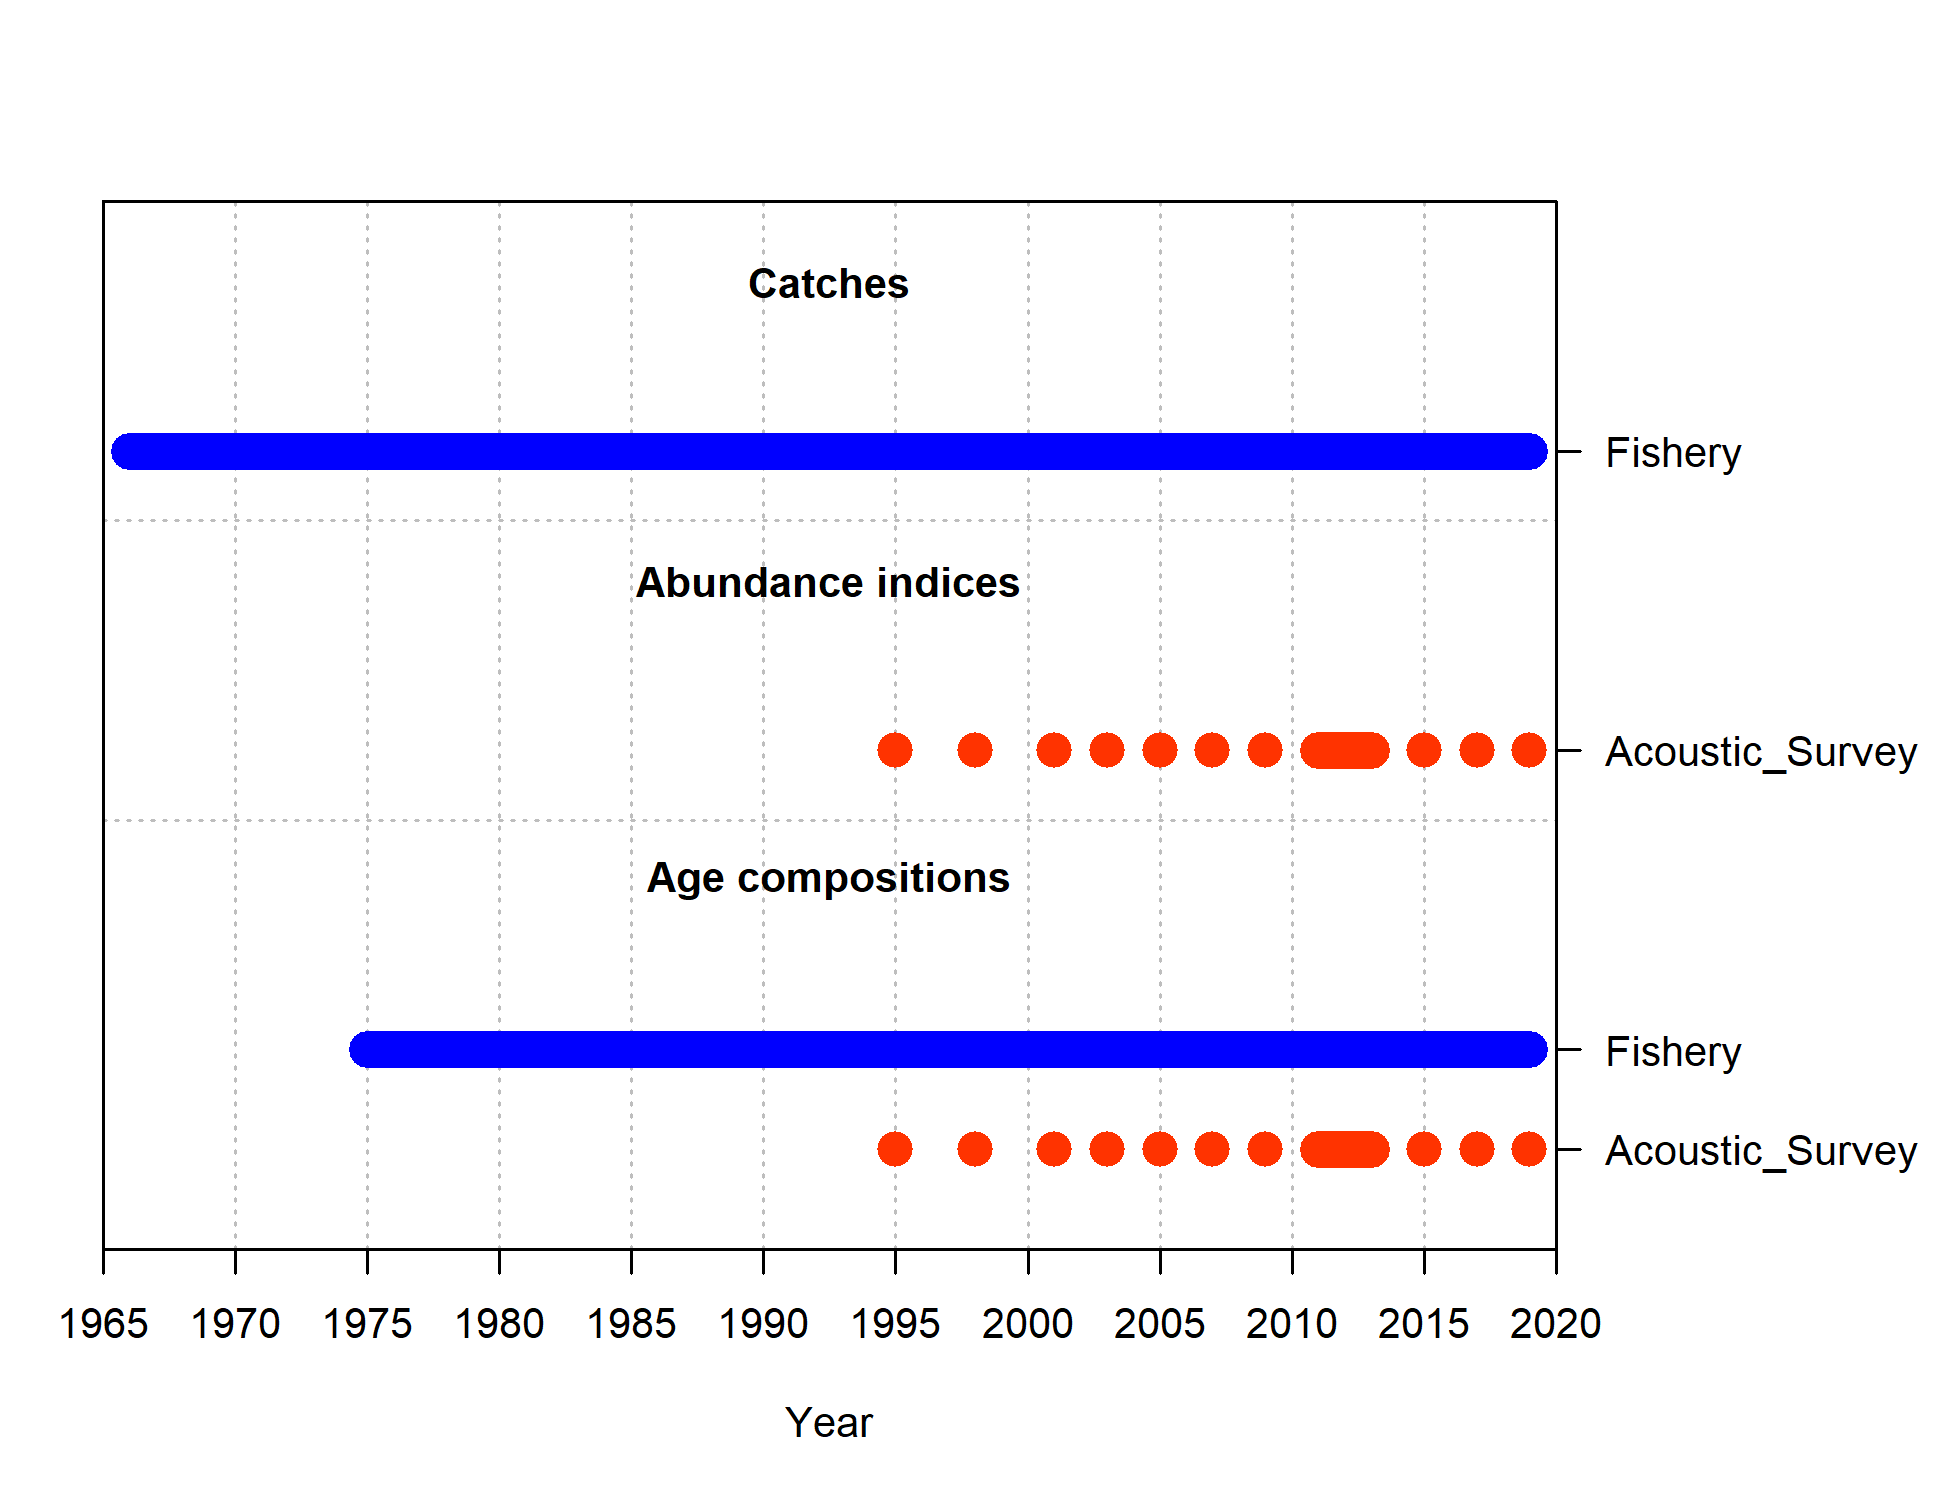
\includegraphics[width=1\textwidth,height=1\textheight]{data-plot.png}
\caption{Summary of data sources used in the base model.\label{fig:data-plot}}
\end{figure}

\tagmcend\tagstructend
\end{document}
